In order to repair malformations of the great arteries surgeons perform several low-level procedures on blood vessels. These include arbitrary incisions, resections of whole blood vessel parts, attaching patches and reconnection of blood vessels end-to-end or end-to-side. From a technical view, all cutting operations can be done prior to simulation by splitting shell elements along their edges which correlates to the actual incision. New shell elements can be added to a mesh or rearranged to align their edges along an incision. On the contrary, joining and suturing of blood vessels and patches typically deform blood vessel walls to a certain amount which has to be simulated. Recent simulation systems \cite{Sorensen2006,Mosegaard2004,Li2009} realize suturing through attachment of contracting springs that have no physical correlation. Springs introduce surplus energy to a physical system and special care has to be taken during simulation to compensate for that.

\begin{figure}[tbh]
\begin{center}
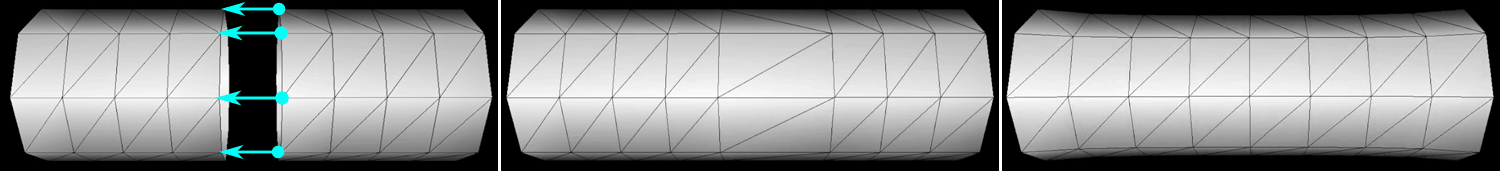
\includegraphics[width=\columnwidth]{img/new-joining.png}
\end{center}
\caption{Joining of thin shell element meshes. Left: Split meshes. Center: Shell elements along the joining edges are connected. Right: Final result after the simulation.}
\label{fig-JoiningVessels}
\end{figure}

We present a new approach that overcomes these difficulties by performing topological changes on the mesh to connect shell elements along joining edges (see figure \ref{fig-JoiningVessels}). Since there is a certain distance between two joining edges in general, a topological modification alters the shape and size of affected shell elements. 
Both actual shape $\myvec{x}$ and rest shape $\myvec{x_0}$ of these shells are modified.
Note that in this simulation state there is temporarily no correlation to reality. 
We then start a controlled relaxation process during which the shell elements progressively converge to their energetical equilibrium
(i.e. we progressively re-contract the rest shape of the shells to their initial value while the simulation computes the deformation of the whole mesh).
To keep the simulation stable we avoid a strong increase in internal forces by linearly interpolating the rest shape of the connected mesh to the initial rest shape before joining. 
The effect is similar to contracting springs but there is no such problem like surplus energy after the joining process is done.


% The primary goal of the surgery is to restore a normal heart function and circulation.
% This goal is reached by rebuilding the heart in a more or less anatomical way.
% There are several types of low-level task the surgeon usually employs while
% performing the surgery that are:

% \begin{description}

  % \item[End to end aortoplasty:] the surgeon completely cuts away the
    % affected part of aorta and sutures the two ends of aorta back together.

  % \item[Patch aortoplasty:] the surgeon performs a cut along the axis of
    % the aorta thus allowing the narrow place to expand. Then applies a
    % patch from artificial material to fill the hole in.

  % \item[Subclavian flap aortoplasty:] the nearest artery is cut,
    % removing also half of the artery (along the axis) and part of the
    % aorta in the affected place. He then uses the rest of the artery to
    % patch the aorta.
    
  % \item[Reconnection and joining of blood vessels:] In addition to the modification of the aorta, the surgeon is lead to establish certain connections that are absent in pathological anatomy.

% \end{description}

% With our method we are able to simulate these tasks, in order to be able to plan them.
% We have based our general approach on a common characteristic: In all these operations the surgeon sutures two or more edges of the vessel walls together.
% Since we are interested in predicting the results rather than creating a training simulator for suturing (trained surgeon knows well how to perform the sutures) the simplest way of performing the suture would be to connect the respective edges with springs. 
% Springs however adds some unwanted energy to the system. 
% Our method is based on a topological connection of the shell elements that are neighbors of the joining edges and a controlled relaxation of these shell elements' rest shape.

% We start with a mesh representing the situation after all the cuts have been performed but before suturing takes place. 
% In the first step we perform the required topological changes to the mesh. We keep the number of elements in new mesh the same as in the original mesh so that we can define 1:1 mapping between elements of these meshes.
% The Figure \ref{fig-JoiningVessels} (a) and (b) explains this operation when joining vessels. 
% Then we start the simulation on the modified mesh while keeping the information of the original rest shapes of all shell elements. 

% \begin{figure}[tbh]
% \begin{center}
% 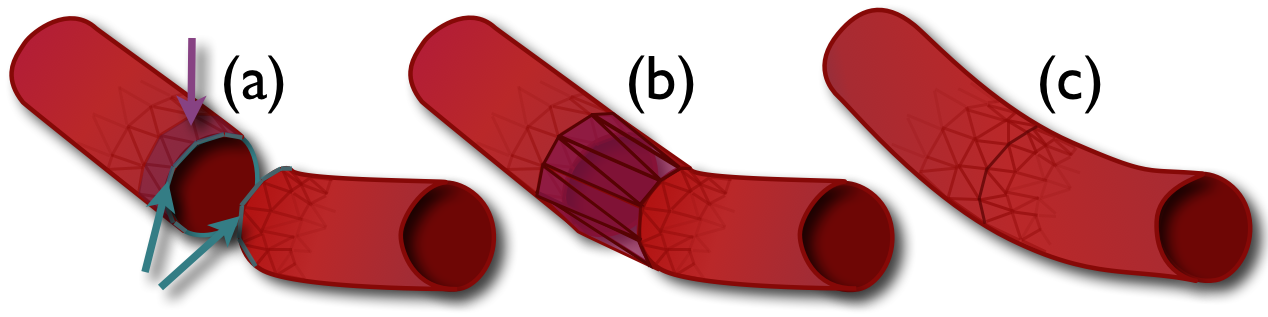
\includegraphics[width=\columnwidth]{img/rest_shape_scheme.png}
% \end{center}

% \caption{Scheme showing the method for joining two vessels \stefan{Isn't that example too complex? I think it is really hard to actually see what is happening here. At least the colors have to be changed because the different layers are colored quite equally and it should be zoomed in to the interesting area were the joining takes place. Remember also that the procedings are printed in black and white and that everything must be visible when printing out this figure black and white. There must be way more contrast.}:  (a) the cut on vessel meshes is performed in a 3D geometry edition software. In the software, we impose that the number of the segments on the edges is the same on both side  (\color{BlueGreen}{$\mathbf{\rightarrow}$}\color{black})
% Moreover, we select some shell elements that lie along the sutured edges (\color{purple}{$\mathbf{\rightarrow}$}\color{black}).
% (b) In our software, we connect the vessel topologies by performing a relaxation of the shape and the rest shape for the selected shells.  
% (c) We progressively re-contract the rest shape of the shells while computing the deformation of the whole unified mesh. 
% In the final steady state computed in the simulation, the shell elements have all their correct rest shape.}
% \label{fig-JoiningVessels}
% \end{figure}

% We can not always step back all the shells to their original shape (transition from figure \ref{fig-JoiningVessels} (b) to (c))  in a single simulation step. 
% In case of non-small distance between the nodes that are sutured together, the involved elements will undergo large deformation that could create quick and non-smooth increase of internal forces and  cause unwanted effects.
% To allevieate the problem we have implemented the technique that allows for moderate changes in the rest shape between simulation steps.
% Between the start and the end of the simulation we use a linear interpolation of the rest shape for the shells that lie along the sutured edges. 
% The interpolation starts with the rest shape equal to the deformed elements and we progressively lead the elements to recover their original rest shape.
% This way, the simulation gradually forces the side edges to connect without any abrupt jump in the behavior.
% When all elements have recover their original rest shape, the steady state found in the simulation corresponds to a physics-based energetical equilibrium of the shells deformation. 
% Thus, we take these positions as an estimation of the result of the connection of the vessels.
